%! Author = joels
%! Date = 13/07/2021

\section{React}
Ist eine Library von Facebook, um User Interfaces zu bauen.\\
\textcolor{b}{\textbf{Prinzipien:}} Komplexes Problem aufteilen in einfachere Komponenten. Bessere Wiederverwendbarkeit, Erweiterbarkeit, Wartbarkeit, Testbarkeit und Aufgabenverteilung\\
\textcolor{b}{\textbf{Komponenten und Elemente:}} Sind Funktionen, die HTML zurückgeben. Beliebige Komposition von React-Elementen und DOM-Elementen:
\subsection{JavaScript XML}
\begin{minipage}{0.4\linewidth}
  React verwendet JSX (blau), eine Erweiterung von JavaScript (gelb). \textbf{Styles} werden nicht als Strings, sondern als Objekt mitgegeben
\end{minipage}
\begin{minipage}{0.6\linewidth}
  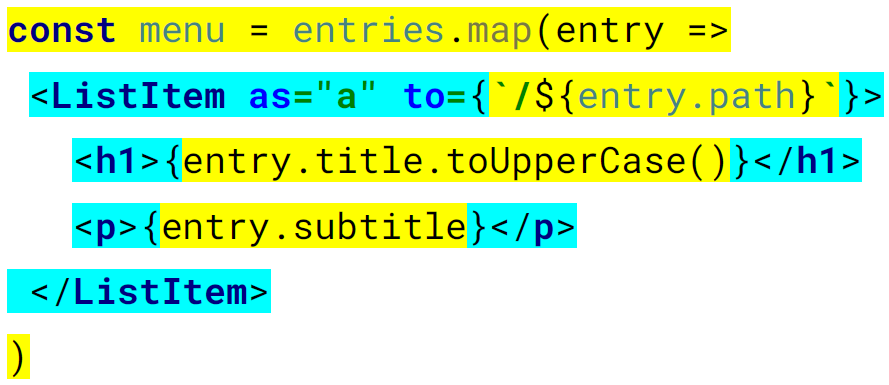
\includegraphics[width=1\linewidth]{jsx.png}
\end{minipage}
\subsubsection{Conditionals}
Was zu null, true, false oder undefined evaluiert wird nicht ausgegeben\\
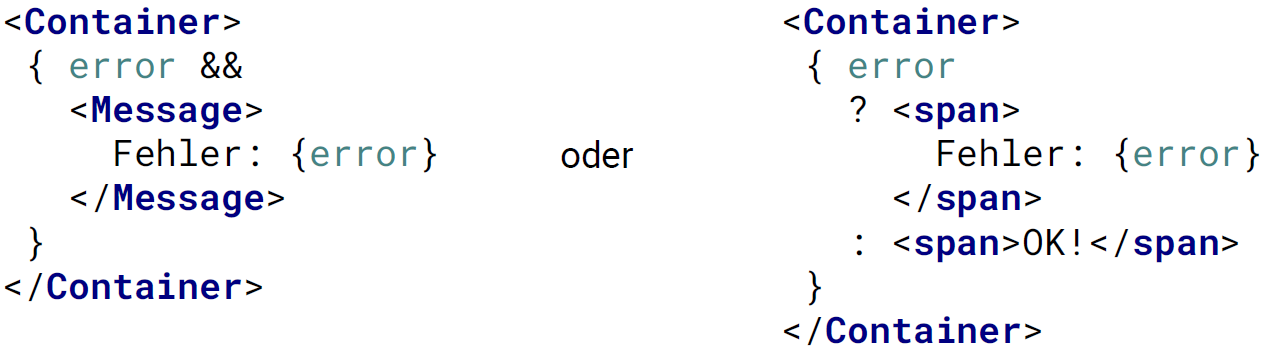
\includegraphics[width=0.73\linewidth]{react_conditional.png}
\subsubsection{Props}
Komponenten erhalten alle Parameter/Properties als \textbf{props} Objekt. Bei Klasse als \textcolor{b}{this.props}, bei Funktionen als Parameter. $\rightarrow$ Props sind immer \textbf{read-only}
\subsection{React State}
React-Klassenkomponenten können einen veränderbaren Zustand haben. Der \textbf{state} einer Komponente ist immer privat. Ändert der State, wird auch die Komponente aktualisiert.
\begin{lstlisting}[style=htmlcssjs]
class Counter extends React.Component {
  state = { counter: 0 }
  increment = () => { this.setState({
    counter: this.state.counter + 1 }) }
  render() { return (<div> {this.state.counter}
    <button onclick={this.increment}>Increment</button>
  </div>) } }
\end{lstlisting}
\subsection{Formulare mit React}
\begin{lstlisting}[style=htmlcssjs]
<form onSubmit={this.handleSubmit}>
<input value={this.state.username} onChange={this.handleUsernameChange}>
</form>
handleUsernameChange = (event) => { this.setState({username: event.target.value}); };
handleSubmit = (event) => { event.preventDefault(); }
\end{lstlisting}
\subsection{Komponenten Lifecycle}
\textcolor{b}{\textbf{Mounting:}}\\
\textbf{1. constructor(props)} $\rightarrow$ State initialisieren, sonst weglassen\\
\textbf{2. static getDerivedStateFromProps(props, state)}\\
$\rightarrow$ Von State abhängige Props initialisieren\\
\textbf{3. render()}\\
\textbf{4. componentDidMount()} $\rightarrow$ DOM ist aufgebaut, Guter Punkt um z.B. Async-Daten zu laden, setState Aufruf führt zu re-rendering\\
\textcolor{b}{\textbf{Updating:}}\\
\textbf{1. static getDerivedStateFromProps(props, state)}\\
$\rightarrow$ Von State abhängige Props aktualisieren\\
\textbf{2. shouldComponentUpdate(nextProps, nextState)}\\
$\rightarrow$ Wird false zurückgegeben wird render übersprungen\\
\textbf{3. render()}\\
\textbf{4. getSnapshotBeforeUpdate(prevProps, prevState)}\\
\textbf{5. componentDidUpdate(prevProps, prevState, snaspshot)} $\rightarrow$ Analog zu componentDidMount, DOM ist aktualisiert\\
\textcolor{b}{\textbf{Unmounting:}}\\
\textbf{1. componentWillUnmount()} $\rightarrow$ Aufräumen\\
\textcolor{b}{\textbf{Error Handling:}}\\
\textbf{1. static getDerivedStateFromError(error)}\\
$\rightarrow$ Error im State abbilden\\
\textbf{2. componentDidCatch(error, info)} $\rightarrow$ Logging, Verhindern, dass Fehler propagiert wird, analog zu catch-Block
\subsection{React Router}
Komponentenbibliothek, Komponenten anzeigen/verstecken abhängig von der URL, Für React Web und React Native
\begin{lstlisting}[style=htmlcssjs]
<Router> // Alle Routen müssen Teil des Routers sein, typischerweise nahe der Root-Komponente
<Route exact path="/" component={Home} /> // Component
//Home wird nur gerendert, wenn der path (exakt) matcht,
//Mehrere Route Elemente können gleichzeitig aktiv sein
<Link to="/">Home</Link> // App-interne Links verwenden nicht <a> sondern <Link>
\end{lstlisting}
\subsection{Hooks}
\textbf{Problem von Lifecycle Methoden:} Zusammengehörender Code ist auf mehrere Methoden verteilt (Mount/Unmount).\\
\textbf{Problem von Klassen-State:} State ist über verschiedene Methoden verteilt\\
\textbf{Fazit:}
\begin{itemize}[topsep=0pt, leftmargin=3mm]
  \setlength\itemsep{-0.3em}
  \item Lifecycle $\&$ State ohne Klassen machen react verständlicher
  \item Klassen sind weiterhin unterstützt
  \item Hooks erlauben, Logik mit Zustand einfacher wiederzuverwenden
\end{itemize}
\textcolor{b}{\textbf{State Hook:}}
\begin{lstlisting}[style=htmlcssjs]
function Counter(){const [count,setCount] = useState(0);
  return(<button onClick={() => setCount( count+1) }>Click me</button>) ;}
\end{lstlisting}
\textcolor{b}{\textbf{Effect Hook:}}
\begin{lstlisting}[style=htmlcssjs]
useEffect(() => { if (!user) {
  fetchAccountDetails(); }
}, [fetchAccountDetails, user]);
\end{lstlisting}
\subsection{Typechecking}
\textcolor{b}{\textbf{Flow:}}
\begin{itemize}[topsep=0pt, leftmargin=3mm]
  \setlength\itemsep{-0.3em}
  \item Erweitert JavaScript um Typenannotationen
  \item Typ-Annotation im Code Typ-Inferenz für lokale Definitio.
  \item Generics, Maybe-Types, Union and Intersection-Types
\end{itemize}
\textcolor{b}{\textbf{TypeScript:}}
\begin{itemize}[topsep=0pt, leftmargin=3mm]
  \setlength\itemsep{-0.3em}
  \item Mehr Typensicherheit in React-Komponenten
  \item Props und State lassen sich typisieren
\end{itemize}
\textcolor{b}{\textbf{Vorteil gegenüber Flow:}}
\begin{itemize}[topsep=0pt, leftmargin=3mm]
  \setlength\itemsep{-0.3em}
  \item Vollwertige Programmiersprache
  \item Besser unterstützt von Libraries und IDEs
  \item TypeScript Fehler müssen korrigiert werden
\end{itemize}
\subsection{Redux}
Library für Statemanagement (Repräsentation, Veränderung, Benachrichtigung). State wird als (immutable) Tree von Objekten dargestellt. Veränderung am Tree führt durch den Reducer zu einem neuen Tree t+1 (funktionale Programmierung).\\
$\rightarrow$ State wird im \textbf{Store} verwaltet.\\
\textcolor{b}{\textbf{Redux Actions:}}\\
Benötigt um Stateänderungen zu machen. Wird an den Store gesendet/dispatched. Ist eine reine Beschreibung der Action.
\begin{lstlisting}[style=htmlcssjs]
{type: 'TRANSFER', amount: 100 }
\end{lstlisting}
\textcolor{b}{\textbf{Redux Reducer-Funktionen:}}\\
Reducer sind pure Funktionen, haben also keine Seiteneffekte.
\begin{lstlisting}[style=htmlcssjs]
function balance(state = 0, action) {
  switch (action.type) { case 'TRANSFER':
    return (state + action.amount);
  default: return state; } }
\end{lstlisting}
\textbf{Reducer kombinieren:} Jeder Reducer erhält einen Teil des States-Trees, für den er zuständig ist. Resultat wird in einem neuen State-Objekt kombiniert.
\begin{lstlisting}[style=htmlcssjs]
function rootReducer(state = {}, action) { return {
  balance: balance(state.balance, action),
  transactions:transactions(state.transactions,action)}}
// Hilfsfunktion combineReducers:
const rootReducer = combineReducers({
  balance, transactions });
\end{lstlisting}
\textcolor{b}{\textbf{Store erstellen:}}\\
Mit dem root-Reducer kann der Store erstellt werden:
\begin{lstlisting}[style=htmlcssjs]
const store = createStore(rootReducer);
\end{lstlisting}
\subsection{Redux mit React verbinden}
\textcolor{b}{\textbf{mapStateToProps:}} Erhält State und kann daraus Props ableiten. Die Komponente bekommt auch die dispatch Methode des Stores als Prop. Das Resultat von connect ist wieder eine React-Komponente, die nun aber mit dem Store verbunden ist (Connected Component)\\
$\rightarrow$ Store muss der Root-Komponente mitgegeben werden.\\
$\rightarrow$ \textbf{Redux Thunk} erlaubt es uns, anstelle eines Objektes eine Funktion zu dispatchen
\begin{lstlisting}[style=htmlcssjs]
const mapStateToProps = (state) => { return {
  transactions: state.transactions } }
const mapDispatchToProps = { fetchTransactions }
export default connect(mapStateToProps, mapDispatchToProps)(Component);
\end{lstlisting}
\subsubsection{Thunk Actions (für asynchrone Funktionen)}
\begin{lstlisting}[style=htmlcssjs]
function fetchTransactions(token) {
  return (dispatch, getState) => {
    dispatch({type: "FETCH_TRANSACTIONS_STARTED"});
    api.getTransactions(token)
      .then(({result: transactions}) => {
        dispatch({type: "FETCH_TRANSACTIONS_SUCCEEDED", transactions}); }) }; }
\end{lstlisting}